\documentclass[journal]{IEEEtran}

\usepackage[T1]{fontenc}
\usepackage[utf8]{inputenc}
\usepackage{amsmath}
\usepackage{booktabs}
\usepackage{tabularx}
\usepackage{array}
\usepackage{graphicx}
\usepackage{microtype}
\usepackage{threeparttable}
\usepackage{enumitem}
\usepackage{url}
\usepackage[hidelinks]{hyperref}
\usepackage{balance}

\graphicspath{{figures/}}
\newcolumntype{Y}{>{\raggedright\arraybackslash}X}

% ================================================================
% VERIFIED STUDY CONSTANTS
% ================================================================
\newcommand{\NSelected}{21,388}
\newcommand{\PSelected}{18,617}
\newcommand{\NExcluded}{411}
\newcommand{\NTrain}{17,084}
\newcommand{\PTrain}{14,823}
\newcommand{\NVal}{2,146}
\newcommand{\PVal}{1,917}
\newcommand{\NTest}{2,158}
\newcommand{\PTest}{1,877}
\newcommand{\TrainMean}{-0.0008252534}
\newcommand{\TrainStd}{0.2322225812}
\newcommand{\BootstrapReps}{5,000}
\newcommand{\BootstrapTotal}{39}
\newcommand{\BootstrapConfidenceBetter}{38}
\newcommand{\BootstrapInconclusive}{1}
\newcommand{\BootstrapAlternativeBetter}{0}

\newcommand{\SeedOneValAUROC}{0.930357}
\newcommand{\SeedTwoValAUROC}{0.928325}
\newcommand{\SeedThreeValAUROC}{0.930900}
\newcommand{\SeedMeanValAUROC}{0.92986}
\newcommand{\SeedSDValAUROC}{0.00136}

\newcommand{\ValAURCConfidence}{0.052765}
\newcommand{\ValAURCLU}{0.057162}
\newcommand{\ValAURCU}{0.059716}
\newcommand{\ValAURCLQU}{0.071156}

\newcommand{\LeadMaskSevereAUROC}{0.810324}
\newcommand{\LeadMaskSevereFone}{0.456728}
\newcommand{\LeadMaskSevereRisk}{0.283967}
\newcommand{\LeadMaskSevereConfidence}{0.843669}
\newcommand{\LeadMaskSevereQ}{0.272734}
\newcommand{\LeadMaskSevereU}{0.019291}

% Exact clean fold-10 values are loaded from the audited reporting tables.
% Run populate_manuscript_results.py inside the audited project before submission.
\InputIfFileExists{paper_values.tex}{}{%
  \newcommand{\CleanTestAUROC}{\texttt{[AUDITED VALUE]}}%
  \newcommand{\CleanTestAP}{\texttt{[AUDITED VALUE]}}%
  \newcommand{\CleanTestFone}{\texttt{[AUDITED VALUE]}}%
  \newcommand{\CleanTestRisk}{\texttt{[AUDITED VALUE]}}%
  \newcommand{\CleanTestConfidenceAURC}{\texttt{[AUDITED VALUE]}}%
  \newcommand{\CleanTestUAURC}{\texttt{[AUDITED VALUE]}}%
  \newcommand{\CleanTestLUAURC}{\texttt{[AUDITED VALUE]}}%
  \newcommand{\CleanTestLQUAURC}{\texttt{[AUDITED VALUE]}}%
}

\title{Identifying Unreliable ECG Predictions: A Stress Test of Confidence, Signal Quality, Annotation Quality, and Model Uncertainty}

\author{Muhammad~Idrees%
\thanks{Add the final author list, affiliations, corresponding author information, funding statement, and CRediT contributions after all authors approve the manuscript.}}

\begin{document}
\maketitle

\begin{abstract}
Deep ECG classifiers can achieve strong average performance while still making individual errors that should be reviewed rather than accepted automatically. The practical problem is deciding which predictions to defer. Ordinary model confidence is a natural choice, but ECG failures can also reflect ambiguous annotations, poor waveform quality, or model uncertainty. We tested whether these additional signals actually improve case-level deferral. Using PTB-XL v1.0.3, we trained a fixed 1-D residual network on patient-disjoint folds 1 to 8, used fold 9 for every development decision, and reserved fold 10 for final evaluation. We compared ordinary confidence with retrospective annotation support, a waveform quality score, Monte Carlo dropout uncertainty, and fixed combinations of these signals. The primary endpoint was area under the risk-coverage curve, where lower values indicate better selective prediction. The same frozen model was evaluated on clean ECGs and under baseline wander, additive white noise, amplitude clipping, and lead masking at three severity levels. Final differences were estimated with \BootstrapReps{} paired patient-level bootstrap replicates. Across \BootstrapTotal{} prespecified comparisons, \BootstrapConfidenceBetter{} had 95\% intervals supporting lower AURC for ordinary confidence, one comparison was inconclusive, and none supported an alternative as better. The main finding is therefore simple: a signal can detect degradation without ranking individual prediction errors better. In this study, annotation quality, signal quality, and model uncertainty described different reliability problems, but ordinary confidence remained the stronger deferral score.
\end{abstract}

\begin{IEEEkeywords}
ECG, PTB-XL, selective prediction, abstention, uncertainty, signal quality, annotation quality, risk-coverage, robustness.
\end{IEEEkeywords}

\section{Introduction}
\IEEEPARstart{D}{eep} learning has substantially improved automated ECG interpretation, especially with large public resources such as PTB-XL \cite{wagner2020ptbxl,strodthoff2021ptbxl}. Most ECG studies, however, are judged by average discrimination or classification performance. That is necessary, but it does not answer a second question that matters whenever a model is used to support clinical decisions: which individual predictions are reliable enough to accept, and which should be sent for additional review?

Selective prediction addresses this question by allowing a model to retain predictions on more reliable cases and defer the remainder \cite{geifman2017selective,geifman2019selectivenet}. A useful deferral score must therefore do more than react when a dataset becomes harder. It must place likely errors earlier in the rejection order so that risk falls as coverage is reduced.

For ECG models, there are several plausible sources of unreliability. The reference annotation itself may be weak or ambiguous. The waveform may contain baseline drift, high-frequency contamination, clipping, or missing leads. The classifier may also be unstable even when the signal appears adequate. These sources are related to different parts of the prediction pipeline, which makes a combined reliability score intuitively attractive. Clinical uncertainty literature has similarly argued that prediction systems should be able to express when they are unsure and defer difficult cases \cite{kompa2021second,chua2023uncertainty}.

The unresolved problem is whether these additional signals actually improve the ranking of individual errors. A waveform quality score can detect a noisy recording while the classifier still predicts it correctly. Model uncertainty can rise across a corrupted cohort while confidence still provides the better ordering of correct and incorrect predictions. Annotation support can identify difficult benchmark labels but is not available for a new unlabeled patient. In other words, detecting that conditions have worsened and identifying which prediction is wrong are not the same task.

This study tests that distinction directly on PTB-XL. The research question is:

\begin{quote}
\textbf{Do annotation quality, waveform quality, and model uncertainty improve selective ECG prediction beyond ordinary predictive confidence, particularly when the ECG signal is degraded?}
\end{quote}

We answer this question using a patient-disjoint development and test design, a fixed raw-waveform classifier, three complementary reliability signals, four controlled corruption families, and patient-level bootstrap inference. All definitions were frozen before the final test was opened. The purpose is not to introduce another ECG architecture. The purpose is to determine whether additional reliability information improves the operational decision to defer an individual prediction.

\begin{figure*}[t]
\centering
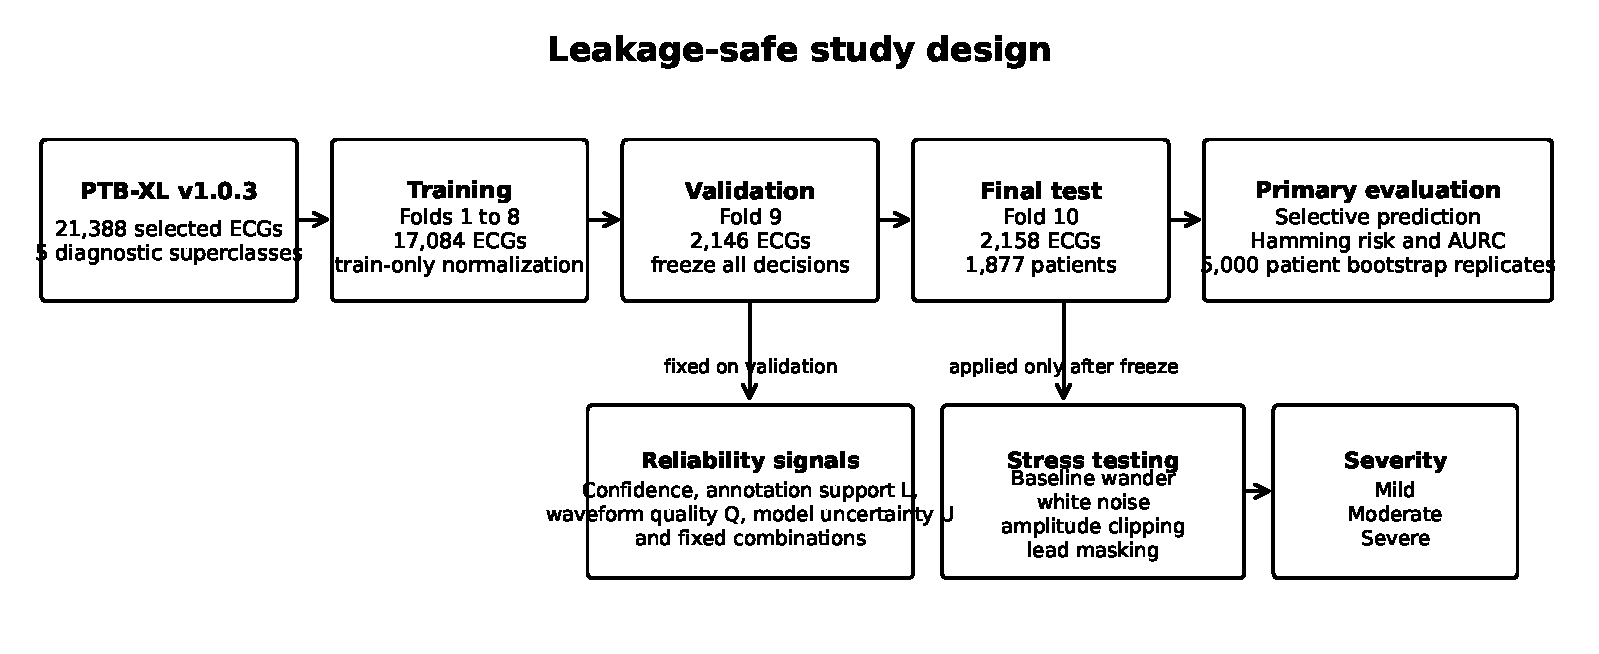
\includegraphics[width=0.98\textwidth]{study_design.pdf}
\caption{Leakage-safe study design. Training, validation, and final test folds were patient-disjoint. All thresholds, reliability definitions, score combinations, and corruption settings were fixed using training and validation information before fold 10 was evaluated.}
\label{fig:study_design}
\end{figure*}

\section{Related Work}
\subsection{ECG Classification and Robustness}
PTB-XL provides 10-second, 12-lead clinical ECGs, diagnostic statements, patient identifiers, and recommended folds for reproducible evaluation \cite{wagner2020ptbxl}. Benchmarking work found that convolutional and residual time-series models are strong baselines for PTB-XL tasks \cite{strodthoff2021ptbxl}. Noise sensitivity remains an important issue because ECG recordings can contain acquisition artifacts and missing information. Prior work has evaluated how noise changes ECG classification performance, including on PTB-XL \cite{bender2023noise}. Our study differs by asking whether reliability signals can identify the individual predictions that should be deferred, not only whether aggregate accuracy changes under noise.

\subsection{Uncertainty and Selective Prediction}
Selective classification evaluates a model together with a rule that decides which predictions to retain \cite{geifman2017selective,geifman2019selectivenet}. In medical AI, uncertainty has been proposed as a way to support abstention, second opinions, and safer use under distribution shift \cite{kompa2021second,chua2023uncertainty,goetz2024generalization}. Monte Carlo dropout is a practical method for obtaining stochastic predictions from an existing network \cite{gal2016dropout}, while broader uncertainty studies have shown that uncertainty quality can deteriorate under shift \cite{ovadia2019shift}. These findings motivate direct evaluation of the deferral decision rather than assuming that a larger uncertainty value is automatically more useful.

\subsection{Study Gap}
Most reliability indicators describe one source of difficulty. Confidence is model-centric, signal-quality measures are input-centric, and annotation metadata are dataset-centric. It is therefore reasonable to expect that combining them might improve reliability assessment. What is less clear is whether such combinations improve case-level selective prediction once the classifier, thresholds, score definitions, and test conditions are fixed. This study isolates that question.

\section{Materials and Methods}
\subsection{Dataset, Targets, and Cohort}
We used PTB-XL version 1.0.3 and only the 100-Hz waveform files. Each ECG contains 1,000 samples for the 12 standard leads. Diagnostic SCP statements were mapped to the five PTB-XL diagnostic superclasses: normal ECG (NORM), myocardial infarction (MI), ST/T change (STTC), conduction disturbance (CD), and hypertrophy (HYP). The task was multilabel, so more than one superclass could be present in a record.

Records without any of these five diagnostic superclasses were excluded. The resulting cohort contained \NSelected{} ECGs from \PSelected{} patients; \NExcluded{} records were excluded by this rule. Among the selected records, 16,244 had one positive superclass, 4,068 had two, 919 had three, and 157 had four.

We followed the PTB-XL fold structure throughout the study. Folds 1 to 8 formed the training set, fold 9 was used for validation and every development decision, and fold 10 was reserved for the final test. Table~\ref{tab:split} gives the exact cohort sizes.

\begin{table}[t]
\centering
\caption{Patient-disjoint study split.}
\label{tab:split}
\begin{tabular}{lrr}
\toprule
Split & ECGs & Patients \\
\midrule
Training, folds 1 to 8 & \NTrain{} & \PTrain{} \\
Validation, fold 9 & \NVal{} & \PVal{} \\
Final test, fold 10 & \NTest{} & \PTest{} \\
\bottomrule
\end{tabular}
\end{table}

\subsection{Preprocessing}
The study used the original 100-Hz signals without resampling, filtering, detrending, notch filtering, clipping, or per-record normalization. A single global mean and standard deviation were estimated from all waveform values in the training split only. The training mean was \TrainMean{} mV and the standard deviation was \TrainStd{} mV. The same fixed transformation was then applied to validation and test ECGs. Extreme values were retained rather than removed after inspecting the training distribution.

For corruption experiments, perturbations were applied to the raw physical waveform first, followed by the same fixed training-derived normalization. This order matters because applying corruption after normalization would change the physical interpretation of the specified SNR and clipping levels.

\subsection{Baseline Classifier and Thresholds}
The classifier was a 1-D residual network from the ResNet1D-Wang family with 473,349 trainable parameters. The input shape was 12 by 1,000 and the output contained five sigmoid probabilities. The architecture served as classifier infrastructure rather than as the contribution of the study.

Training used binary cross-entropy, AdamW, maximum learning rate 0.01, weight decay 0.01, a One-Cycle learning-rate schedule, batch size 128, and 50 epochs. The checkpoint with the highest validation macro-AUROC was retained. The main development seed was 20260826. Two additional seeds, 20260827 and 20260828, were run after the protocol had been frozen to quantify training reproducibility. These runs did not use test records for training or checkpoint selection.

Class-specific decision thresholds were chosen on fold 9 by maximizing F1 and then frozen. The thresholds were 0.527930 for NORM, 0.342066 for MI, 0.420363 for STTC, 0.512351 for CD, and 0.191394 for HYP. No threshold was fitted or adjusted on fold 10.

\subsection{Reliability Signals}
The study compared ordinary confidence with three additional reliability signals. Their purpose and limitations are summarized in Table~\ref{tab:signals} and Fig.~\ref{fig:signals}. The signals were intentionally kept separate because they do not measure the same phenomenon.

\begin{figure*}[t]
\centering
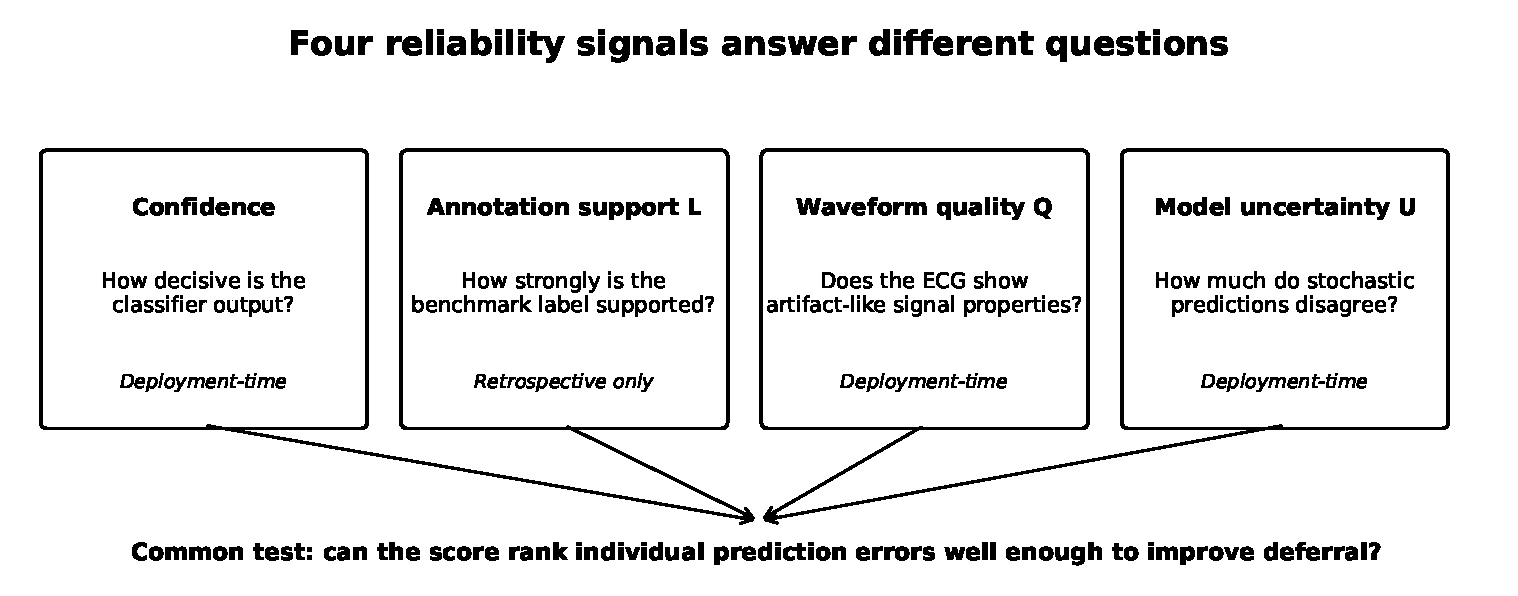
\includegraphics[width=0.97\textwidth]{reliability_signals.pdf}
\caption{Interpretation of the four reliability signals. The primary evaluation did not ask whether a signal increased when conditions became worse. It asked whether the signal ranked individual prediction errors well enough to improve deferral.}
\label{fig:signals}
\end{figure*}

\begin{table*}[t]
\centering
\caption{Reliability signals evaluated in the study.}
\label{tab:signals}
\begin{tabularx}{\textwidth}{p{2.2cm}Y Y p{2.4cm}}
\toprule
Signal & Question represented by the score & Operational definition & Availability \\
\midrule
Confidence & How decisive is the classifier output? & For each of the five labels, the probability assigned to the predicted binary outcome was taken; the five values were averaged. Higher values indicate stronger model confidence. & Deployment-time \\
\addlinespace
Annotation support, $L$ & How strongly is the benchmark diagnosis supported? & For each positive superclass, the strongest available diagnostic SCP likelihood was retained and then averaged across positive superclasses. A likelihood of 0 was treated as unavailable, not as zero confidence. Records without an available value used the frozen validation median. & Retrospective only \\
\addlinespace
Waveform quality, $Q$ & Does the ECG show artifact-like signal properties? & Four raw-signal features captured baseline-frequency burden, high-frequency burden, lead dropout, and clipping. Each was converted to a training-reference badness percentile, then averaged and inverted so that higher $Q$ indicates a cleaner signal. & Deployment-time \\
\addlinespace
Model uncertainty, $U$ & How much do stochastic model predictions disagree? & Thirty MC-dropout passes were run with batch normalization fixed in evaluation mode and only the two existing head dropout layers active. Per-class mutual information was computed and averaged across the five labels. Higher values indicate greater stochastic disagreement. & Deployment-time \\
\bottomrule
\end{tabularx}
\end{table*}

The waveform quality score was designed to capture artifact-like properties rather than disease-related amplitude. Baseline-frequency burden used the largest lead-wise power fraction from 0.1 to 1 Hz relative to 0.1 to 50 Hz. High-frequency burden used the corresponding 40 to 50 Hz fraction. Lead-dropout burden compared the smallest lead AC RMS with the median AC RMS across leads. Clipping burden measured the largest lead-wise fraction of samples exactly at the observed signal minimum or maximum. Constant leads received maximal clipping burden. Leads with zero total spectral power were excluded from spectral ratios instead of assigning an artificial ratio through an epsilon denominator. A record with zero spectral power in all 12 leads was treated as invalid. For this reason, $Q$ should be interpreted as a study-specific relative waveform quality score, not as a clinically validated universal signal-quality index.

For $U$, 30 stochastic forward passes were used. The score was the mean classwise mutual information between the predictive distribution and the stochastic dropout predictions. We use this as an MC-dropout uncertainty indicator. It should not be interpreted as an exact Bayesian posterior measure of epistemic uncertainty.

\subsection{Combining the Signals}
The numerical scales of $L$, $Q$, and $U$ are different. Before combining them, each was placed in a common badness direction and converted to an empirical midrank percentile using the validation reference distribution only. The transformations used $1-L$, $1-Q$, and $U$. Pairwise and three-way combinations were simple equal-weight averages of these percentiles. No combination weight was optimized.

Eight selection scores were evaluated: confidence, $L$, $Q$, $U$, $L+Q$, $L+U$, $Q+U$, and $L+Q+U$. The three comparisons specified in advance for patient-level inference were $L+U$ versus confidence, $U$ versus confidence, and $L+Q+U$ versus confidence. The test distribution was never used to fit percentile mappings or combination weights.

\subsection{Selective Prediction Endpoint}
The primary unit of error was one ECG record. For each record, Hamming error was the proportion of the five frozen binary decisions that were incorrect. A record with one wrong superclass decision therefore had a Hamming error of 0.2, while a record with all five decisions correct had error 0.

For each reliability score, records were ranked from most to least reliable. Coverage is the fraction of ECGs retained, and risk is the mean Hamming error among those retained ECGs. The risk-coverage curve therefore measures whether deferring low-ranked cases actually removes errors. Its area, AURC, was the primary endpoint, with lower values indicating a better deferral score. Exact score ties were handled as groups so that equal values were not assigned an arbitrary order. Random ordering has expected AURC equal to full-coverage mean risk. An oracle ranking was calculated only as a diagnostic reference and was never used for tuning.

\subsection{Signal Corruption Protocol}
The final model was evaluated on clean ECGs and 12 corrupted conditions. Four corruption families were used at three severities each, as shown in Table~\ref{tab:corruptions}. Random perturbations were deterministic per ECG under the frozen study seed.

\begin{table*}[t]
\centering
\caption{Prespecified signal corruptions. Perturbations were applied to the raw waveform before the fixed training-derived normalization.}
\label{tab:corruptions}
\begin{tabularx}{\textwidth}{p{3.0cm}Y p{3.4cm}}
\toprule
Corruption & Definition & Mild / Moderate / Severe \\
\midrule
Baseline wander & A 0.2-Hz sinusoid was added with an independently sampled phase for each lead. Its amplitude was scaled to a target per-lead SNR. & 18 / 12 / 6 dB \\
Additive white noise & Zero-mean Gaussian noise was scaled independently for each lead to a target SNR. & 18 / 12 / 6 dB \\
Amplitude clipping & Each lead was clipped symmetrically around its own mean using the centered absolute-amplitude quantile. & 99.5 / 97.5 / 95.0 percentile \\
Lead masking & A deterministic set of leads was replaced by a flat 0-mV signal. & 1 / 3 / 6 leads \\
\bottomrule
\end{tabularx}
\end{table*}

The SNR values were chosen to provide mild, moderate, and severe stress levels and overlap values used in ECG noise stress testing \cite{moody1984noise}. These perturbations are controlled synthetic tests. They are not intended to reproduce every real acquisition artifact or every hospital environment.

\subsection{Secondary Metrics and Statistical Analysis}
Secondary classification metrics were macro-AUROC, macro-average precision, macro-F1, and Brier score. The primary selective-prediction endpoint remained AURC.

For each of the 13 final test conditions, the prespecified comparison was the alternative method's AURC minus the confidence AURC. Positive differences therefore favor ordinary confidence because lower AURC is better. Uncertainty in each difference was estimated with \BootstrapReps{} paired patient-clustered bootstrap replicates using seed 20260826. Patients, not ECG records, were sampled with replacement. When a patient was drawn more than once, all ECGs from that patient received the same multiplicity. This preserved within-patient dependence and kept every method comparison paired on the same resampled cohort.

We report condition-specific 95\% percentile intervals. These 39 intervals were not multiplicity-adjusted, so they are not presented as family-wise corrected significance tests. The main interpretation is whether the uncertainty interval for a prespecified comparison lies entirely above zero, entirely below zero, or crosses zero.

\subsection{Protocol Freeze and Integrity Checks}
Before fold 10 was evaluated, the model checkpoint, preprocessing statistics, classification thresholds, definitions of $L$, $Q$, and $U$, validation percentile references, score combinations, corruption settings, and primary bootstrap comparisons were frozen. No method was redesigned after the final test results were inspected.

The reporting pipeline was then checked against the frozen artifacts. The final audit verified source hashes, record and patient identities, unchanged targets across conditions, array shapes, bootstrap point differences, seed-level checkpoint reproduction, and generated reporting hashes. All 299 audit checks passed. The automated test suite also passed 118 of 118 tests.

\section{Results}
\subsection{Training Was Reproducible Across Seeds}
The three training runs produced best validation macro-AUROC values of \SeedOneValAUROC{}, \SeedTwoValAUROC{}, and \SeedThreeValAUROC{}. Their mean was \SeedMeanValAUROC{} with sample standard deviation \SeedSDValAUROC{}. The best epochs were 26, 19, and 17, respectively. Both additional reproducibility runs reported zero test records used during training or checkpoint selection.

\begin{figure}[t]
\centering

\includegraphics[width=\columnwidth]{seed_reproducibility.pdf}
\caption{Best validation macro-AUROC across the three prespecified training seeds. The narrow spread indicates that baseline validation performance was not dependent on one favorable initialization.}
\label{fig:seeds}
\end{figure}

\begin{table}[t]
\centering
\caption{Training reproducibility.}
\label{tab:seeds}
\begin{tabular}{lcc}
\toprule
Seed & Best epoch & Macro-AUROC \\
\midrule
20260826 & 26 & \SeedOneValAUROC{} \\
20260827 & 19 & \SeedTwoValAUROC{} \\
20260828 & 17 & \SeedThreeValAUROC{} \\
\midrule
Mean $\pm$ SD & not applicable & \SeedMeanValAUROC{} $\pm$ \SeedSDValAUROC{} \\
\bottomrule
\end{tabular}
\end{table}

\subsection{Validation Did Not Justify Retuning}
Before the final test was opened, ordinary confidence already had the lowest clean validation AURC among the main scores considered for inference. Confidence achieved \ValAURCConfidence{}, compared with \ValAURCLU{} for $L+U$, \ValAURCU{} for $U$, and \ValAURCLQU{} for $L+Q+U$. We therefore retained the prespecified definitions without changing the quality score, uncertainty estimator, percentile mappings, or combination weights.

\subsection{Clean Held-Out Test Performance}
The final test contained \NTest{} ECGs from \PTest{} patients. Table~\ref{tab:clean_test} reports the clean classification and selective-prediction results. The values are loaded directly from the audited reporting files by the supplied manuscript population script, which prevents a validation number from being copied accidentally into a test result.

\begin{table}[t]
\centering
\caption{Clean fold-10 test performance.}
\label{tab:clean_test}
\begin{tabular}{lc}
\toprule
Metric & Value \\
\midrule
Macro-AUROC & \CleanTestAUROC{} \\
Macro-average precision & \CleanTestAP{} \\
Macro-F1 & \CleanTestFone{} \\
Full-coverage Hamming risk & \CleanTestRisk{} \\
Confidence AURC & \CleanTestConfidenceAURC{} \\
\bottomrule
\end{tabular}
\end{table}

\InputIfFileExists{generated_classwise_table.tex}{}

\subsection{Ordinary Confidence Was the Stronger Deferral Score}
The primary result is shown in Fig.~\ref{fig:forest}. Across the \BootstrapTotal{} prespecified method-condition comparisons, \BootstrapConfidenceBetter{} had 95\% bootstrap intervals entirely above zero. In these comparisons, the alternative had higher AURC than ordinary confidence. One interval crossed zero, and no interval lay entirely below zero. Thus, none of the three prespecified alternatives had condition-specific bootstrap support for lower AURC than confidence in any tested condition.

\begin{figure*}[t]
\centering
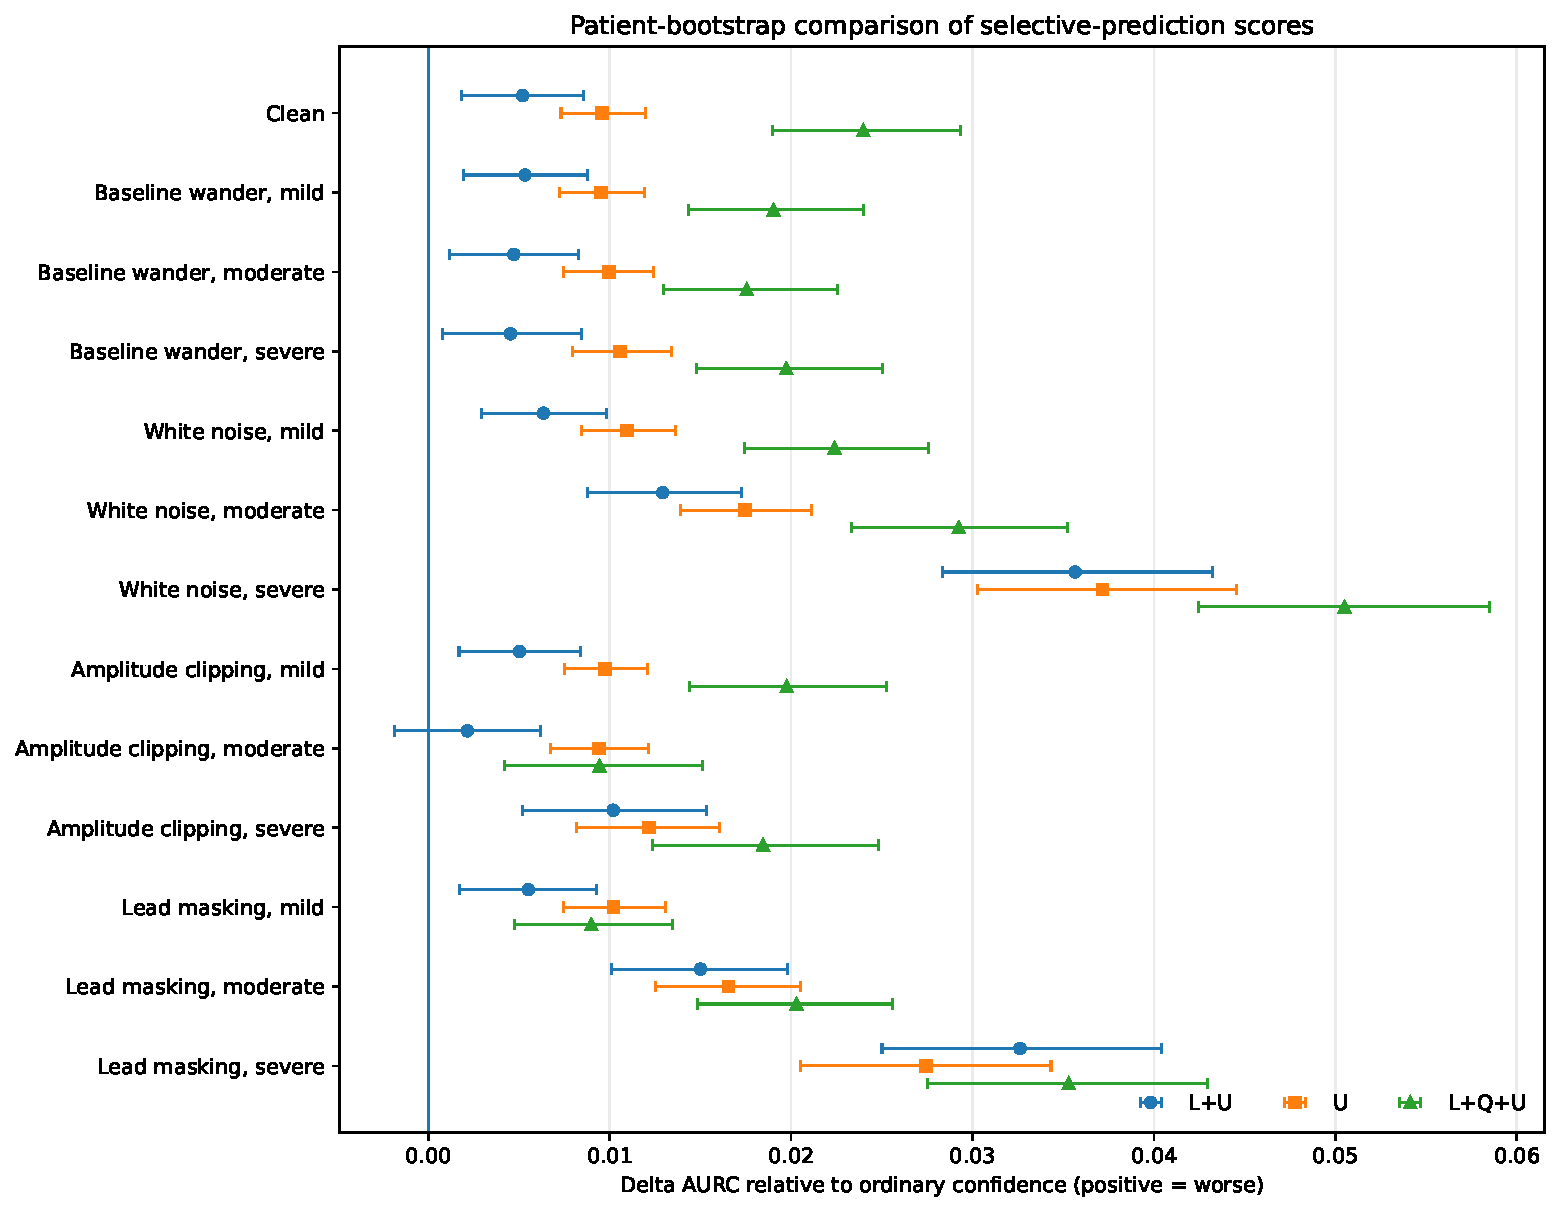
\includegraphics[width=0.93\textwidth]{bootstrap_forest_all39.pdf}
\caption{All 39 prespecified patient-level bootstrap comparisons. Each point is the alternative AURC minus the ordinary-confidence AURC. Positive values favor ordinary confidence because lower AURC is better. Error bars are condition-specific 95\% percentile bootstrap intervals. Only $L+U$ under moderate amplitude clipping crosses zero.}
\label{fig:forest}
\end{figure*}

On clean test data, the AURC difference was 0.005202 for $L+U$ with 95\% CI [0.001855, 0.008580], 0.009577 for $U$ with CI [0.007315, 0.011949], and 0.023986 for $L+Q+U$ with CI [0.018973, 0.029342]. The only inconclusive comparison was $L+U$ under moderate amplitude clipping, where the difference was 0.002151 with CI [-0.001878, 0.006166]. Under severe white noise, the corresponding differences increased to 0.035658, 0.037177, and 0.050502, and all three intervals remained above zero. The complete 39 comparisons are reported in Appendix~\ref{app:bootstrap}.

\subsection{Corruption Increased Error, but Degradation Detection Did Not Equal Error Ranking}
The corruption experiments explain why additional signals did not automatically improve selective prediction. In the frozen validation analysis, mean $U$ increased monotonically with severity for all four corruption families. Mean ordinary confidence decreased monotonically, and full-coverage Hamming risk increased monotonically, for all four families. The waveform quality score $Q$ decreased monotonically for baseline wander and amplitude clipping, but not for white noise or lead masking. Thus, several reliability indicators changed in the expected direction as conditions worsened, yet their case-level rankings still produced higher AURC than confidence.

The held-out severe lead-masking condition illustrates this distinction. Macro-AUROC fell to \LeadMaskSevereAUROC{}, macro-F1 to \LeadMaskSevereFone{}, and full-coverage Hamming risk rose to \LeadMaskSevereRisk{}. Mean confidence was \LeadMaskSevereConfidence{}, mean $Q$ was \LeadMaskSevereQ{}, and mean $U$ was \LeadMaskSevereU{}. Despite clear degradation and higher model uncertainty, the patient-bootstrap AURC differences for $L+U$, $U$, and $L+Q+U$ were all positive with intervals above zero.

\IfFileExists{figures/corruption_hamming_risk.pdf}{%
\begin{figure}[t]
\centering
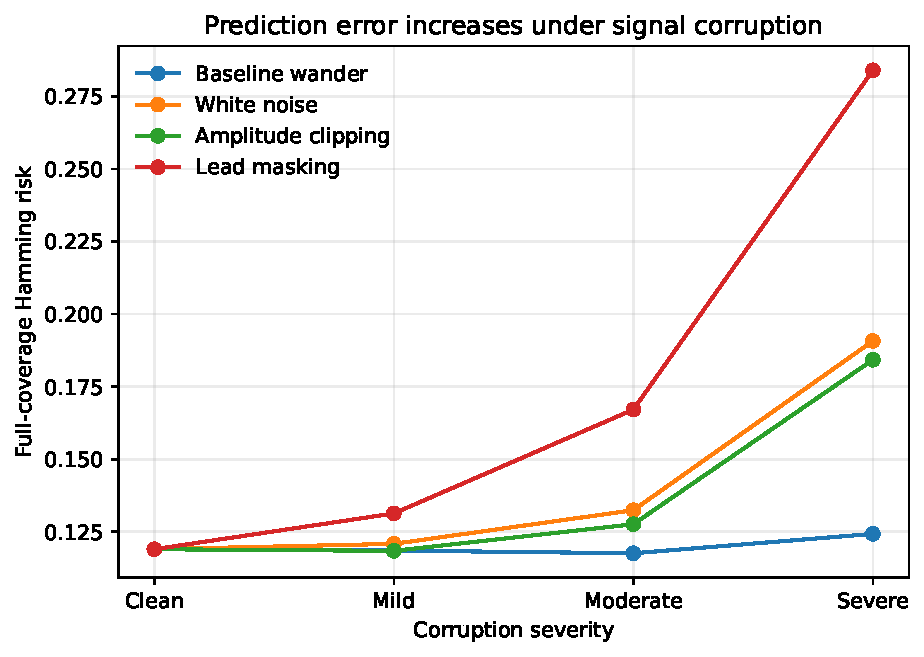
\includegraphics[width=\columnwidth]{corruption_hamming_risk.pdf}
\caption{Held-out full-coverage Hamming risk across corruption severity. This figure is generated directly from the audited fold-10 condition table.}
\label{fig:corruption_risk}
\end{figure}}{}

\IfFileExists{figures/corruption_mean_uncertainty.pdf}{%
\begin{figure}[t]
\centering
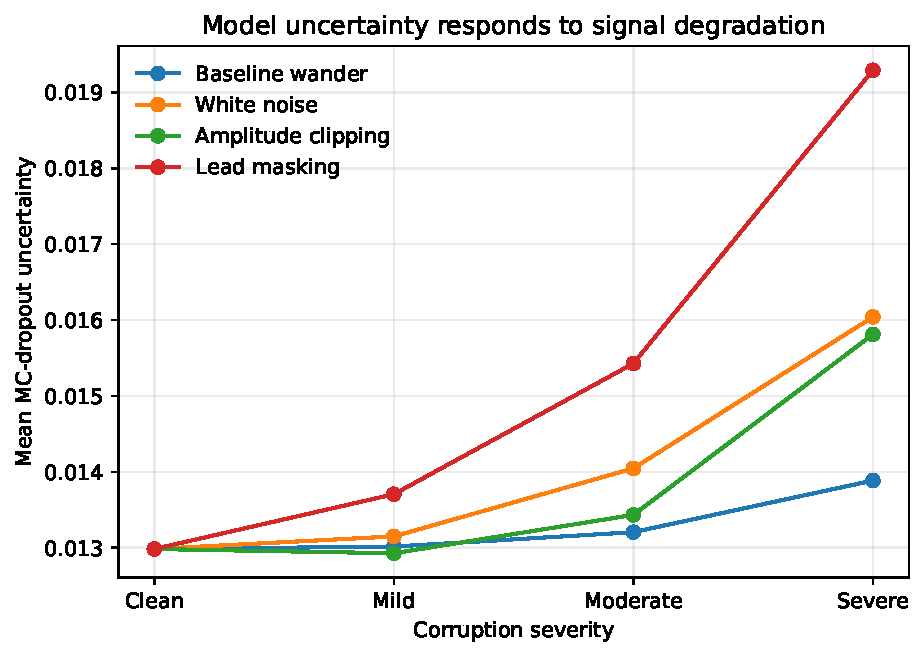
\includegraphics[width=\columnwidth]{corruption_mean_uncertainty.pdf}
\caption{Mean MC-dropout uncertainty across corruption severity on fold 10. This figure is generated directly from the audited condition table.}
\label{fig:corruption_u}
\end{figure}}{}

\section{Discussion}
\subsection{Main Finding}
The study began with a plausible hypothesis. If an ECG prediction is supported by a strong annotation, a clean waveform, and a stable model, combining these signals might identify unreliable predictions better than model confidence alone. The final results did not support that hypothesis. Ordinary confidence remained the stronger selective-prediction score on clean data and across the tested corruptions. Of 39 prespecified patient-level comparisons, 38 had intervals supporting lower AURC for confidence, one was inconclusive, and none supported an alternative as better.

This is not the same as saying that $L$, $Q$, or $U$ are useless. Their value depends on what decision they are meant to support. The key result is that detecting a reliability problem and ranking individual classifier errors are different tasks.

\subsection{Why the Additional Signals Did Not Improve Deferral}
Ordinary confidence is directly linked to the classifier's output margin. If many errors occur near that margin, confidence can already rank difficult cases effectively. The other signals are more indirect. A low-quality ECG can still contain enough information for an easy diagnosis. A record with weaker annotation support can still be predicted consistently. MC-dropout disagreement can increase when a cohort is corrupted without identifying the same individual cases that the deterministic classifier gets wrong.

The fixed equal-weight combinations can also dilute a strong ranking signal. We deliberately did not optimize weights after observing the test results. A learned referral model might produce a different outcome, but it would answer a different research question and would require a new development and evaluation protocol.

\subsection{Implications for Medical AI Reliability}
Reliability metrics should be validated against the action they are expected to trigger. If the goal is acquisition monitoring, a waveform quality score can be useful even when it is not the best deferral score. If the goal is cohort monitoring, a rise in MC-dropout uncertainty can signal that operating conditions have changed. If the goal is benchmark curation, retrospective annotation support can identify labels that deserve review. None of these uses requires the signal to outperform confidence for case-level abstention.

For selective prediction, the relevant endpoint is whether rejecting lower-ranked cases actually reduces prediction error at a useful coverage. This is why risk-coverage behavior is more informative for deferral than uncertainty magnitude alone. The distinction is especially important in medical AI, where uncertainty is often discussed as a safety mechanism \cite{kompa2021second,chua2023uncertainty,goetz2024generalization}.

\subsection{Strengths}
The main strength of the study is methodological control. The dataset split was patient-disjoint. Normalization parameters were estimated from training data only. All thresholds and reliability definitions were fixed before the final test. Corruptions were applied in physical units before normalization. Score ties were treated as groups in the risk-coverage calculation. The final uncertainty analysis resampled patients rather than individual ECGs. Most importantly, the method was not redesigned after the final results failed to support the initial hypothesis. The complete computational chain was then verified by 299 integrity checks and 118 automated tests.

\subsection{Limitations}
The study has several limitations. First, the final evaluation is an internal patient-disjoint PTB-XL test rather than an external hospital cohort, so the results do not establish cross-institutional generalization. Second, the four corruption families are controlled synthetic perturbations. The 0.2-Hz baseline sinusoid, Gaussian white noise, quantile-based clipping, and flat lead masking do not reproduce the complete distribution of real acquisition artifacts.

Third, $Q$ is a training-referenced relative quality score developed for this experiment and is not a clinically validated universal ECG signal-quality index. Fourth, $L$ is retrospective and depends on annotation metadata, so it cannot be computed for a truly unlabeled deployment ECG. Fifth, $U$ is derived from the two dropout modules already present in the model head. It is therefore a practical MC-dropout indicator, not a complete Bayesian representation of epistemic uncertainty. Sixth, Hamming risk weights the five binary label decisions equally. A clinical deployment may assign different costs to different diagnoses, false negatives, and false positives. Seventh, the reported 95\% bootstrap intervals are condition-specific and were not adjusted across the 39 comparisons. Finally, the findings apply to these frozen signals and equal-weight combinations. They do not establish that every ensemble, conformal method, uncertainty estimator, learned referral model, or task-specific signal-quality measure would fail to improve on confidence.

\section{Conclusion}
We tested a simple but important question: can additional reliability information identify unreliable ECG predictions better than ordinary confidence? In this PTB-XL study, annotation support, waveform quality, and MC-dropout uncertainty captured different aspects of reliability and reacted to different forms of degradation, but they did not improve case-level selective prediction. Ordinary confidence had lower AURC with 95\% bootstrap intervals above zero in 38 of 39 prespecified comparisons, one comparison was inconclusive, and none favored an alternative. The broader lesson is that a signal that detects degradation is not necessarily a signal that ranks individual errors well. Reliability measures should therefore be judged against the decision they are intended to support.

\appendices
\section{Complete Bootstrap Comparisons}
\label{app:bootstrap}
\begin{table*}[h]
\centering
\scriptsize
\caption{Complete patient-bootstrap AURC comparisons. Each cell reports alternative AURC minus confidence AURC with its 95\% percentile interval. Positive values favor ordinary confidence because lower AURC is better.}
\label{tab:all_bootstrap}
\begin{tabular}{lccc}
\toprule
Condition & $L+U$ vs. confidence & $U$ vs. confidence & $L+Q+U$ vs. confidence \\
\midrule
Clean & 0.005202 [0.001855, 0.008580] & 0.009577 [0.007315, 0.011949] & 0.023986 [0.018973, 0.029342] \\
Baseline wander, mild & 0.005333 [0.001920, 0.008778] & 0.009533 [0.007208, 0.011907] & 0.019039 [0.014361, 0.023985] \\
Baseline wander, moderate & 0.004718 [0.001155, 0.008258] & 0.009948 [0.007475, 0.012395] & 0.017560 [0.012940, 0.022544] \\
Baseline wander, severe & 0.004532 [0.000784, 0.008422] & 0.010575 [0.007934, 0.013387] & 0.019732 [0.014806, 0.025049] \\
White noise, mild & 0.006345 [0.002913, 0.009829] & 0.010951 [0.008433, 0.013605] & 0.022388 [0.017452, 0.027560] \\
White noise, moderate & 0.012921 [0.008783, 0.017264] & 0.017447 [0.013883, 0.021125] & 0.029230 [0.023329, 0.035239] \\
White noise, severe & 0.035658 [0.028369, 0.043205] & 0.037177 [0.030275, 0.044529] & 0.050502 [0.042477, 0.058522] \\
Amplitude clipping, mild & 0.005027 [0.001694, 0.008407] & 0.009742 [0.007531, 0.012075] & 0.019753 [0.014399, 0.025262] \\
Amplitude clipping, moderate & 0.002151 [-0.001878, 0.006166] & 0.009401 [0.006718, 0.012138] & 0.009442 [0.004213, 0.015102] \\
Amplitude clipping, severe & 0.010196 [0.005190, 0.015342] & 0.012165 [0.008174, 0.016039] & 0.018457 [0.012378, 0.024830] \\
Lead masking, mild & 0.005511 [0.001696, 0.009247] & 0.010222 [0.007450, 0.013073] & 0.008990 [0.004746, 0.013454] \\
Lead masking, moderate & 0.015002 [0.010094, 0.019805] & 0.016540 [0.012522, 0.020493] & 0.020290 [0.014821, 0.025574] \\
Lead masking, severe & 0.032617 [0.025010, 0.040415] & 0.027444 [0.020535, 0.034327] & 0.035308 [0.027497, 0.042958] \\
\bottomrule
\end{tabular}
\end{table*}

\section{Complete Condition-Level Test Metrics}
\InputIfFileExists{generated_condition_table.tex}{%
}{%
The supplied population script generates the complete clean and corruption table directly from the audited fold-10 condition metrics file. This prevents manual transcription of test values.}

\section*{Data Availability}
PTB-XL version 1.0.3 is publicly available through PhysioNet. The final submitted manuscript should include the permanent dataset citation and the exact archived analysis version used for this study.

\section*{Code Availability}
The frozen configurations, analysis code, hashes, automated test outputs, and reporting artifacts should be deposited in a permanent public archive before submission. Replace this paragraph with the final repository DOI or permanent URL.

\section*{Ethics Statement}
This study used publicly available de-identified PTB-XL data and collected no new participant data. The ethics and consent procedures for the original dataset are described by Wagner \emph{et al.} \cite{wagner2020ptbxl}.

\section*{Competing Interests}
The authors declare no competing interests. Confirm this statement with all co-authors before submission.

\section*{Funding}
Insert the exact funding statement agreed by all authors and institutions.

\section*{Author Contributions}
Insert the final CRediT contribution statement after the author list is confirmed.

\balance
\begin{thebibliography}{99}

\bibitem{wagner2020ptbxl}
P. Wagner, N. Strodthoff, R.-D. Bousseljot, D. Kreiseler, F. I. Lunze, W. Samek, and T. Schaeffter, ``PTB-XL, a large publicly available electrocardiography dataset,'' \emph{Scientific Data}, vol. 7, art. no. 154, 2020, doi: 10.1038/s41597-020-0495-6.

\bibitem{strodthoff2021ptbxl}
N. Strodthoff, P. Wagner, T. Schaeffter, and W. Samek, ``Deep Learning for ECG Analysis: Benchmarks and Insights from PTB-XL,'' \emph{IEEE Journal of Biomedical and Health Informatics}, vol. 25, no. 5, pp. 1519--1528, 2021, doi: 10.1109/JBHI.2020.3022989.

\bibitem{geifman2017selective}
Y. Geifman and R. El-Yaniv, ``Selective Classification for Deep Neural Networks,'' in \emph{Advances in Neural Information Processing Systems}, vol. 30, 2017.

\bibitem{geifman2019selectivenet}
Y. Geifman and R. El-Yaniv, ``SelectiveNet: A Deep Neural Network with an Integrated Reject Option,'' in \emph{Proceedings of the 36th International Conference on Machine Learning}, vol. 97, pp. 2151--2159, 2019.

\bibitem{kompa2021second}
B. Kompa, J. Snoek, and A. L. Beam, ``Second opinion needed: communicating uncertainty in medical machine learning,'' \emph{npj Digital Medicine}, vol. 4, art. no. 4, 2021, doi: 10.1038/s41746-020-00367-3.

\bibitem{chua2023uncertainty}
M. Chua \emph{et al.}, ``Tackling prediction uncertainty in machine learning for healthcare,'' \emph{Nature Biomedical Engineering}, vol. 7, pp. 711--718, 2023, doi: 10.1038/s41551-022-00988-x.

\bibitem{goetz2024generalization}
L. Goetz \emph{et al.}, ``Generalization: a key challenge for responsible AI in patient-facing clinical applications,'' \emph{npj Digital Medicine}, vol. 7, art. no. 126, 2024, doi: 10.1038/s41746-024-01127-3.

\bibitem{gal2016dropout}
Y. Gal and Z. Ghahramani, ``Dropout as a Bayesian Approximation: Representing Model Uncertainty in Deep Learning,'' in \emph{Proceedings of the 33rd International Conference on Machine Learning}, vol. 48, pp. 1050--1059, 2016.

\bibitem{ovadia2019shift}
Y. Ovadia \emph{et al.}, ``Can You Trust Your Model's Uncertainty? Evaluating Predictive Uncertainty Under Dataset Shift,'' in \emph{Advances in Neural Information Processing Systems}, vol. 32, 2019.

\bibitem{bender2023noise}
T. Bender, P. Gemke, E. Idrobo-Avila, H. Dathe, D. Krefting, and N. Spicher, ``Benchmarking the Impact of Noise on Deep Learning-Based Classification of Atrial Fibrillation in 12-Lead ECG,'' \emph{Studies in Health Technology and Informatics}, vol. 302, pp. 977--981, 2023, doi: 10.3233/SHTI230321.

\bibitem{moody1984noise}
G. B. Moody, W. E. Muldrow, and R. G. Mark, ``A noise stress test for arrhythmia detectors,'' in \emph{Computers in Cardiology}, vol. 11, pp. 381--384, 1984.

\end{thebibliography}
\end{document}
